
\documentclass[12pt]{article}
\usepackage{amsmath, amssymb, geometry, multicol, enumitem, array, booktabs}
\usepackage[most]{tcolorbox}
\usepackage{xcolor, fancyhdr, tikz}
\usetikzlibrary{arrows.meta, decorations.pathreplacing}

\geometry{margin=0.85in, top=0.7in, bottom=0.85in}

\definecolor{navy}{RGB}{10,36,99}
\definecolor{gold}{RGB}{195,150,30}
\definecolor{teal}{RGB}{0,120,110}
\definecolor{violet}{RGB}{90,30,140}
\definecolor{crimson}{RGB}{160,30,40}
\definecolor{sage}{RGB}{60,140,80}
\definecolor{midgray}{RGB}{110,110,110}
\definecolor{lightgray}{RGB}{242,242,242}
\definecolor{ansgreen}{RGB}{0,130,60}
\definecolor{exbg}{RGB}{235,248,245}

\tcbuselibrary{skins, breakable}

\newtcolorbox{partbox}[2]{%
  enhanced, breakable,
  colback=#1!7, colframe=#1, coltitle=white,
  fonttitle=\bfseries\large,
  title={#2},
  arc=5pt, boxrule=1.5pt,
  left=10pt, right=10pt, top=7pt, bottom=7pt}

\newtcolorbox{exbox}[1]{%
  enhanced, breakable,
  colback=exbg, colframe=teal, coltitle=white,
  fonttitle=\bfseries,
  title={#1},
  arc=5pt, boxrule=1.4pt,
  left=10pt, right=10pt, top=7pt, bottom=8pt}

\newtcolorbox{keybox}{%
  enhanced,
  colback=navy!6, colframe=navy, coltitle=white,
  fonttitle=\bfseries,
  title={Key Rule \textemdash{} Solving $|E| = c$},
  arc=5pt, boxrule=1.4pt,
  left=10pt, right=10pt, top=7pt, bottom=7pt}

\pagestyle{fancy}
\fancyhf{}
\fancyhead[L]{\textcolor{navy}{\bfseries Solving Absolute Value Equations --- Practice}}
\fancyhead[R]{\textcolor{midgray}{\small Score:\;\underline{\hspace{2cm}}}}
\fancyfoot[C]{\textcolor{midgray}{\small\thepage}}
\renewcommand{\headrulewidth}{1.6pt}
\renewcommand{\headrule}{\hbox to\headwidth{\color{navy}\leaders\hrule height\headrulewidth\hfill}}

\newcommand{\wsp}{\vspace{2.6cm}}
\newcommand{\wspm}{\vspace{2.0cm}}
\newcommand{\blank}{\underline{\hspace{2.8cm}}}
\newcommand{\sblank}{\underline{\hspace{1.6cm}}}
\newcommand{\ans}[1]{{\color{ansgreen}\bfseries #1}}

%% ── Number line macro ─────────────────────────────────────────────────────────
%% \numline{min}{max}{step}{dot1/col1, dot2/col2, ...}{label list}
%% Simplified: just draw the axis and let content be in tikzpicture
\newcommand{\numlinebase}[2]{%
  \begin{tikzpicture}[x=0.7cm, y=1cm,
      dot/.style={circle, fill, inner sep=2.2pt},
      arr/.style={-{Stealth[length=5pt]}, thick}]
    \draw[arr] (#1-0.5, 0) -- (#2+0.5, 0);
    \foreach \x in {#1,...,#2} {
      \draw (\x, 0.08) -- (\x, -0.08);
      \node[below, font=\small] at (\x, -0.08) {$\x$};
    }
}

\begin{document}

%% ─── HEADER ───────────────────────────────────────────────────────────────────
\begin{tcolorbox}[enhanced, arc=6pt,
  colback=navy, colframe=gold, boxrule=2.5pt,
  left=12pt, right=12pt, top=10pt, bottom=10pt]
  \begin{center}
    {\color{gold}\fontsize{20}{24}\selectfont\bfseries
      Solving Absolute Value Equations}\\[4pt]
    {\color{white}\small Beginner Practice Sheet \quad|\quad
     Study the examples first, then try the problems!}
  \end{center}
\end{tcolorbox}

\vspace{6pt}

%% ─── Student info ─────────────────────────────────────────────────────────────
\begin{tcolorbox}[colback=lightgray, colframe=midgray, arc=3pt, boxrule=0.8pt,
  left=8pt, right=8pt, top=5pt, bottom=5pt]
\begin{tabular}{p{6cm} p{4cm} p{4cm}}
Name:\;\underline{\hspace{5cm}} &
Date:\;\underline{\hspace{2.8cm}} &
Period:\;\underline{\hspace{2cm}}
\end{tabular}
\end{tcolorbox}

\vspace{10pt}

%% ─── Key Rule ─────────────────────────────────────────────────────────────────
\begin{keybox}
\begin{center}
\renewcommand{\arraystretch}{1.5}
\begin{tabular}{>{\bfseries\color{navy}}p{3.2cm} p{9.5cm}}
Case 1: $c > 0$ & $|E| = c \;\Longrightarrow\; E = c \;\text{ or }\; E = -c$ \quad\textit{(two solutions)}\\
Case 2: $c = 0$ & $|E| = 0 \;\Longrightarrow\; E = 0$ \quad\textit{(one solution)}\\
Case 3: $c < 0$ & $|E| = c \;\Longrightarrow\;$ \textbf{No solution}
\end{tabular}
\end{center}
\vspace{4pt}
\textbf{3 Steps:}\quad
\textcircled{1}~Isolate~$|\cdot|$\quad
\textcircled{2}~Split into two equations\quad
\textcircled{3}~Solve each one
\end{keybox}

\vspace{12pt}

%% ══════════════════════════════════════════════════════════════════════════════
%%  WORKED EXAMPLES
%% ══════════════════════════════════════════════════════════════════════════════

\begin{exbox}{Worked Example 1 \quad Solve $|x| = 4$}

\textbf{What it means:} $|x| = 4$ says ``$x$ is \textbf{4 units away from 0}'' on the number line.
Because distance works in both directions, there are \textbf{two answers}.

\vspace{8pt}
\textbf{Step \textcircled{1}:} The absolute value is already isolated.\quad $|x| = 4$ \checkmark

\vspace{4pt}
\textbf{Step \textcircled{2}:} Split into two equations:
\[
  x = 4 \qquad \text{or} \qquad x = -4
\]

\textbf{Step \textcircled{3}:} Both are already solved. \quad
\fbox{$x = 4 \quad \text{or} \quad x = -4$}

\vspace{10pt}
\textbf{Check on the number line} --- both dots are exactly 4 units from 0:

\vspace{8pt}
\begin{center}
\begin{tikzpicture}[x=0.75cm, y=1cm]
  % axis
  \draw[-{Stealth[length=5pt]}, thick] (-6.3,0) -- (6.3,0);
  % ticks and labels
  \foreach \x in {-6,-5,-4,-3,-2,-1,0,1,2,3,4,5,6} {
    \draw (\x,0.1) -- (\x,-0.1);
    \node[below, font=\footnotesize] at (\x,-0.1) {$\x$};
  }
  % zero label on axis
  % dots
  \filldraw[teal]  (4,0) circle (4pt) node[above=4pt, font=\small\bfseries, color=teal] {$x=4$};
  \filldraw[violet](-4,0) circle (4pt) node[above=4pt, font=\small\bfseries, color=violet] {$x=-4$};
  % distance braces
  \draw[{Stealth[length=4pt]}-{Stealth[length=4pt]}, crimson, thick]
    (-4, -0.55) -- (0, -0.55);
  \node[below, font=\small, color=crimson] at (-2,-0.55) {4 units};
  \draw[{Stealth[length=4pt]}-{Stealth[length=4pt]}, crimson, thick]
    (0, -0.55) -- (4, -0.55);
  \node[below, font=\small, color=crimson] at (2,-0.55) {4 units};
  % center mark
  \filldraw[gold] (0,0) circle (2.5pt);
  \node[above=4pt, font=\small, color=gold] at (0,0) {center};
\end{tikzpicture}
\end{center}

\vspace{4pt}
\textbf{Solution set:} $\{-4,\ 4\}$
\end{exbox}

\vspace{14pt}

\begin{exbox}{Worked Example 2 \quad Solve $|x - 3| + 1 = 6$}

\textbf{What it means:} We need to \textbf{isolate the absolute value first} (Step \textcircled{1}),
then use the distance idea.

\vspace{8pt}
\textbf{Step \textcircled{1}:} Subtract 1 from both sides to isolate $|x-3|$:
\[
  |x - 3| + 1 - 1 = 6 - 1 \qquad\Longrightarrow\qquad |x - 3| = 5
\]

\textbf{Step \textcircled{2}:} $|x-3| = 5$ says ``$x$ is \textbf{5 units from 3}.'' Split:
\[
  x - 3 = 5 \qquad \text{or} \qquad x - 3 = -5
\]

\textbf{Step \textcircled{3}:} Add 3 to each equation:
\[
  x = 8 \qquad\text{or}\qquad x = -2
\]
\fbox{$x = 8 \quad\text{or}\quad x = -2$}

\vspace{10pt}
\textbf{Check on the number line} --- both dots are exactly 5 units from the center 3:

\vspace{8pt}
\begin{center}
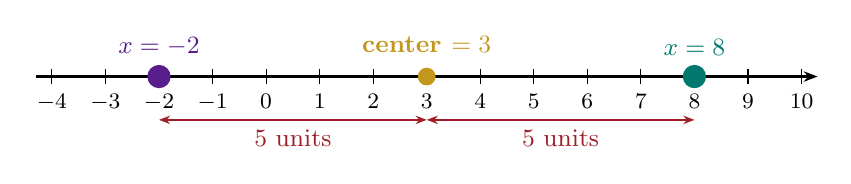
\begin{tikzpicture}[x=0.68cm, y=1cm]
  \draw[-{Stealth[length=5pt]}, thick] (-4.3,0) -- (10.3,0);
  \foreach \x in {-4,-3,-2,-1,0,1,2,3,4,5,6,7,8,9,10} {
    \draw (\x,0.1) -- (\x,-0.1);
    \node[below, font=\footnotesize] at (\x,-0.1) {$\x$};
  }
  % center
  \filldraw[gold] (3,0) circle (3pt);
  \node[above=5pt, font=\small\bfseries, color=gold] at (3,0) {center $= 3$};
  % solutions
  \filldraw[teal]  (8,0) circle (4pt) node[above=4pt,font=\small\bfseries,color=teal] {$x=8$};
  \filldraw[violet](-2,0) circle (4pt) node[above=4pt,font=\small\bfseries,color=violet] {$x=-2$};
  % distance arrows
  \draw[{Stealth[length=4pt]}-{Stealth[length=4pt]}, crimson, thick]
    (-2,-0.55) -- (3,-0.55);
  \node[below, font=\small, color=crimson] at (0.5,-0.55) {5 units};
  \draw[{Stealth[length=4pt]}-{Stealth[length=4pt]}, crimson, thick]
    (3,-0.55) -- (8,-0.55);
  \node[below, font=\small, color=crimson] at (5.5,-0.55) {5 units};
\end{tikzpicture}
\end{center}

\vspace{4pt}
\textbf{Solution set:} $\{-2,\ 8\}$
\end{exbox}

\newpage

%% ══════════════════════════════════════════════════════════════════════════════
%%  PART A — Level 1
%% ══════════════════════════════════════════════════════════════════════════════
\begin{partbox}{teal}{Part A \quad Level 1 --- Direct Absolute Value
  \hfill{\normalfont\small $|x| = c$}}

\textit{Just like Example 1. The answer is $x = c$ or $x = -c$.}
\vspace{8pt}
\begin{multicols}{2}
\begin{enumerate}[label=\textbf{\arabic*.}, itemsep=0pt]

  \item $|x| = 3$\\[3pt]
  Step \textcircled{2}: $x = \sblank$ or $x = \sblank$\\[3pt]
  \textbf{Answer:} \blank
  \wspm

  \item $|x| = 8$\\[3pt]
  Step \textcircled{2}: $x = \sblank$ or $x = \sblank$\\[3pt]
  \textbf{Answer:} \blank
  \wspm

  \item $|x| = 0$\\[3pt]
  \textit{(Hint: $c = 0$, one answer)}\\[3pt]
  \textbf{Answer:} \blank
  \wspm

  \item $|x| = -4$\\[3pt]
  \textit{(Hint: can distance be negative?)}\\[3pt]
  \textbf{Answer:} \blank
  \wspm

  \item $|x| = 1$\\[3pt]
  Step \textcircled{2}: $x = \sblank$ or $x = \sblank$\\[3pt]
  \textbf{Answer:} \blank
  \wspm

  \item $|x| = 10$\\[3pt]
  Step \textcircled{2}: $x = \sblank$ or $x = \sblank$\\[3pt]
  \textbf{Answer:} \blank
  \wspm

\end{enumerate}
\end{multicols}
\end{partbox}

\vspace{12pt}

%% ══════════════════════════════════════════════════════════════════════════════
%%  PART B — Level 2
%% ══════════════════════════════════════════════════════════════════════════════
\begin{partbox}{violet}{Part B \quad Level 2 --- Shift Inside
  \hfill{\normalfont\small $|x \pm a| = c$}}

\textit{Split into two cases, solve for $x$ in each.}
\vspace{8pt}
\begin{multicols}{2}
\begin{enumerate}[label=\textbf{\arabic*.}, itemsep=0pt]

  \item $|x - 2| = 5$\\[3pt]
  $x - 2 = \sblank$ or $x - 2 = \sblank$\\[3pt]
  $x = \sblank$ \hspace{0.9cm} $x = \sblank$\\[3pt]
  \textbf{Answer:} \blank
  \wsp

  \item $|x + 3| = 4$\\[3pt]
  $x + 3 = \sblank$ or $x + 3 = \sblank$\\[3pt]
  $x = \sblank$ \hspace{0.9cm} $x = \sblank$\\[3pt]
  \textbf{Answer:} \blank
  \wsp

  \item $|x - 1| = 6$\\[3pt]
  $x - 1 = \sblank$ or $x - 1 = \sblank$\\[3pt]
  $x = \sblank$ \hspace{0.9cm} $x = \sblank$\\[3pt]
  \textbf{Answer:} \blank
  \wsp

  \item $|x + 5| = 5$\\[3pt]
  $x + 5 = \sblank$ or $x + 5 = \sblank$\\[3pt]
  $x = \sblank$ \hspace{0.9cm} $x = \sblank$\\[3pt]
  \textbf{Answer:} \blank
  \wsp

  \item $|x - 4| = 0$\\[3pt]
  \textit{(One answer only --- why?)}\\[3pt]
  $x - 4 = \sblank \;\Rightarrow\; x = \sblank$\\[3pt]
  \textbf{Answer:} \blank
  \wsp

  \item $|x + 1| = 7$\\[3pt]
  $x + 1 = \sblank$ or $x + 1 = \sblank$\\[3pt]
  $x = \sblank$ \hspace{0.9cm} $x = \sblank$\\[3pt]
  \textbf{Answer:} \blank
  \wsp

\end{enumerate}
\end{multicols}
\end{partbox}

\newpage

%% ══════════════════════════════════════════════════════════════════════════════
%%  PART C — Level 3
%% ══════════════════════════════════════════════════════════════════════════════
\begin{partbox}{gold}{Part C \quad Level 3 --- Isolate First!
  \hfill{\normalfont\small Get $|\cdot|$ alone, then split}}

\textit{Add / subtract / divide to isolate the absolute value first (just like Example 2).}
\vspace{8pt}
\begin{multicols}{2}
\begin{enumerate}[label=\textbf{\arabic*.}, itemsep=0pt]

  \item $|x| + 3 = 7$\\[3pt]
  Step \textcircled{1}: $|x| = \sblank$\\[3pt]
  Step \textcircled{2}: $x = \sblank$ or $x = \sblank$\\[3pt]
  \textbf{Answer:} \blank
  \wsp

  \item $|x - 2| + 1 = 6$\\[3pt]
  Step \textcircled{1}: $|x-2| = \sblank$\\[3pt]
  $x - 2 = \sblank$ or $x - 2 = \sblank$\\[3pt]
  $x = \sblank$ \hspace{0.9cm} $x = \sblank$\\[3pt]
  \textbf{Answer:} \blank
  \wsp

  \item $2|x| = 10$\\[3pt]
  Step \textcircled{1}: $|x| = \sblank$\\[3pt]
  Step \textcircled{2}: $x = \sblank$ or $x = \sblank$\\[3pt]
  \textbf{Answer:} \blank
  \wsp

  \item $2|x + 3| = 8$\\[3pt]
  Step \textcircled{1}: $|x+3| = \sblank$\\[3pt]
  $x + 3 = \sblank$ or $x + 3 = \sblank$\\[3pt]
  $x = \sblank$ \hspace{0.9cm} $x = \sblank$\\[3pt]
  \textbf{Answer:} \blank
  \wsp

  \item $|x + 2| - 3 = 1$\\[3pt]
  Step \textcircled{1}: $|x+2| = \sblank$\\[3pt]
  $x + 2 = \sblank$ or $x + 2 = \sblank$\\[3pt]
  $x = \sblank$ \hspace{0.9cm} $x = \sblank$\\[3pt]
  \textbf{Answer:} \blank
  \wsp

  \item $3|x| = 9$\\[3pt]
  Step \textcircled{1}: $|x| = \sblank$\\[3pt]
  Step \textcircled{2}: $x = \sblank$ or $x = \sblank$\\[3pt]
  \textbf{Answer:} \blank
  \wsp

\end{enumerate}
\end{multicols}
\end{partbox}

\vspace{12pt}

%% ══════════════════════════════════════════════════════════════════════════════
%%  PART D — Challenge
%% ══════════════════════════════════════════════════════════════════════════════
\begin{partbox}{crimson}{Part D \quad Challenge
  \hfill{\normalfont\small Show all steps for both cases}}
\vspace{6pt}
\begin{enumerate}[label=\textbf{\arabic*.}, itemsep=10pt]

  \item $|2x - 4| = 6$
  \vspace{0.4cm}

  \begin{tabular}{p{6.2cm} p{6.2cm}}
  \textbf{Case 1:} $2x - 4 = 6$ & \textbf{Case 2:} $2x - 4 = -6$ \\[6pt]
  $2x = \sblank$ & $2x = \sblank$ \\[6pt]
  $x = \sblank$ & $x = \sblank$
  \end{tabular}

  \vspace{0.3cm}
  \textbf{Answer:} \blank

  \vspace{0.5cm}
  \item $|3x + 3| = 9$
  \vspace{0.4cm}

  \begin{tabular}{p{6.2cm} p{6.2cm}}
  \textbf{Case 1:} $3x + 3 = 9$ & \textbf{Case 2:} $3x + 3 = -9$ \\[6pt]
  $3x = \sblank$ & $3x = \sblank$ \\[6pt]
  $x = \sblank$ & $x = \sblank$
  \end{tabular}

  \vspace{0.3cm}
  \textbf{Answer:} \blank

  \vspace{0.5cm}
  \item $|2x + 1| = 5$
  \vspace{0.4cm}

  \begin{tabular}{p{6.2cm} p{6.2cm}}
  \textbf{Case 1:} \underline{\hspace{5cm}} & \textbf{Case 2:} \underline{\hspace{5cm}} \\[10pt]
  \underline{\hspace{5cm}} & \underline{\hspace{5cm}} \\[10pt]
  $x = \sblank$ & $x = \sblank$
  \end{tabular}

  \vspace{0.3cm}
  \textbf{Answer:} \blank

  \vspace{0.5cm}
  \item $|4x - 8| = 0$
  \hfill{\small\itshape Hint: only one answer!}

  \vspace{2.5cm}
  \textbf{Answer:} \blank

\end{enumerate}
\end{partbox}

%% ══════════════════════════════════════════════════════════════════════════════
%%  ANSWER KEY
%% ══════════════════════════════════════════════════════════════════════════════
\newpage

\begin{tcolorbox}[enhanced, arc=5pt,
  colback=sage!10, colframe=sage, coltitle=white,
  fonttitle=\bfseries\large,
  title={\quad Answer Key \quad (Teacher Copy)},
  boxrule=1.5pt, left=10pt, right=10pt, top=8pt, bottom=8pt]

\textbf{\color{teal}Part A}
\begin{multicols}{3}
\begin{enumerate}[label=\textbf{\arabic*.}, itemsep=3pt]
  \item \ans{$x = 3$ or $x = -3$}
  \item \ans{$x = 8$ or $x = -8$}
  \item \ans{$x = 0$}
  \item \ans{No solution}
  \item \ans{$x = 1$ or $x = -1$}
  \item \ans{$x = 10$ or $x = -10$}
\end{enumerate}
\end{multicols}

\vspace{6pt}\textbf{\color{violet}Part B}
\begin{multicols}{3}
\begin{enumerate}[label=\textbf{\arabic*.}, itemsep=3pt]
  \item \ans{$x = 7$ or $x = -3$}
  \item \ans{$x = 1$ or $x = -7$}
  \item \ans{$x = 7$ or $x = -5$}
  \item \ans{$x = 0$ or $x = -10$}
  \item \ans{$x = 4$}
  \item \ans{$x = 6$ or $x = -8$}
\end{enumerate}
\end{multicols}

\vspace{6pt}\textbf{\color{gold}Part C}
\begin{multicols}{3}
\begin{enumerate}[label=\textbf{\arabic*.}, itemsep=3pt]
  \item \ans{$x = 4$ or $x = -4$}
  \item \ans{$x = 7$ or $x = -3$}
  \item \ans{$x = 5$ or $x = -5$}
  \item \ans{$x = 1$ or $x = -7$}
  \item \ans{$x = 2$ or $x = -6$}
  \item \ans{$x = 3$ or $x = -3$}
\end{enumerate}
\end{multicols}

\vspace{6pt}\textbf{\color{crimson}Part D}
\begin{multicols}{2}
\begin{enumerate}[label=\textbf{\arabic*.}, itemsep=3pt]
  \item \ans{$x = 5$ or $x = -1$}
  \item \ans{$x = 2$ or $x = -4$}
  \item \ans{$x = 2$ or $x = -3$}
  \item \ans{$x = 2$}
\end{enumerate}
\end{multicols}

\end{tcolorbox}

\end{document}
